
%----------------------------------------------------------------------------------------
%	PREAMBUŁA
%----------------------------------------------------------------------------------------

\documentclass[12pt]{article}
\usepackage[polish]{babel}
\usepackage{polski}
\usepackage[utf8]{inputenc}
\usepackage{graphicx}
\usepackage{fancyhdr}
\usepackage{float}
\usepackage{graphicx}
\usepackage[hidelinks]{hyperref}
\usepackage{verbatim}
\usepackage{amsmath}
\usepackage{rotating}
\usepackage{listings}
\usepackage{xcolor}
\usepackage{subcaption}
\usepackage{vmargin}
\setmarginsrb{2 cm}{2 cm}{2 cm}{2 cm}{1 cm}{1.5 cm}{1 cm}{1.5 cm}


\definecolor{lgray}{gray}{0.96}
\definecolor{lbcolor}{rgb}{0.9,0.9,0.9}
\lstset{
    framesep=2pt,
    breaklines=true,
    breakatwhitespace=true,
    basicstyle=\footnotesize,
    aboveskip={0.75\baselineskip},
    columns=flexible,
    showstringspaces=false,
    breaklines=true,
    prebreak = \raisebox{0ex}[0ex][0ex]{\ensuremath{\hookleftarrow}},
    frame=single,
    rulecolor=\color{lgray},
    showtabs=false,
    showspaces=false,
    showstringspaces=false,
    backgroundcolor=\color{lgray},
    identifierstyle=\ttfamily,
    keywordstyle=\color[rgb]{0,0,1},
    commentstyle=\color[rgb]{0.0,0.26,0.15},
    stringstyle=\color[rgb]{0.627,0.126,0.941}
}

\graphicspath{{static/}} 

\title{Sztuczne Sieci Neuronowe - Projekt}
\author{Aleksandra Poręba, Grzegorz Podsiadło}

\makeatletter
\let\thetitle\@title
\let\theauthor\@author
\let\thedate\@date
\makeatother

%----------------------------------------------------------------------------------------
%	STRONA TYTUŁOWA
%----------------------------------------------------------------------------------------
\begin{document}
\begin{center}
\textsc{\normalsize Wydział Fizyki i Informatyki Stosowanej}\\[2.0cm] 
\includegraphics[scale = 1]{logo.pdf}\\[1cm] 
\textsc{\Large Sztuczne Sieci Neuronowe}\\[0.4cm] 


{ \huge \bfseries \LARGE{Sprawozdanie z projektu} } 

\flushright \Large Aleksandra Poręba \\ Grzegorz Podsiadło

\vfill 

\center {\today}\\[2cm] 


\pagebreak 

\end{center}

%----------------------------------------------------------------------------------------
%	SPIS TREŚCI
%----------------------------------------------------------------------------------------
\setcounter{tocdepth}{2}
\tableofcontents
\pagebreak

%----------------------------------------------------------------------------------------
%	ZAWARTOŚĆ
%----------------------------------------------------------------------------------------

\pagestyle{fancy}
\fancyhf{}

\rhead{\theauthor}
\lhead{\thetitle}
\cfoot{\thepage}

\section{Wstęp}

\pagebreak
\section{Poszukiwanie konfiguracji sieci neuronowej}
% że regresja, co testowaliśmy i dlaczego takie
% mlp 

Przetestowano konfigurację sieci o jednej oraz dwóch warstwach, z wykorzystaniem różnych kombinacji funkcji:
\begin{enumerate}
\item \verb+logsig+
\item \verb+tansig+
\item \verb+purelin+
\item \verb+radbas+
\end{enumerate}
Dla każdej konfiguracji zbadano również wpływ ilości neuronów w poszczególnych warstwach. Ilość neuronów zmieniano między  10 a 100 ze skokiem 10. Wykresy błędów dla wybranych konfiguracji znajdują się na następnych stronach.


\begin{figure}[H]
\centering
\begin{subfigure}[t]{0.48\textwidth} 
\centering
\includegraphics[height=2.2in]{purelin_purelin_20_learn.png}
\caption{MSE uczenia dla 20 neuronów.}
\end{subfigure}
~~
\begin{subfigure}[t]{0.48\textwidth} 
\centering
\includegraphics[height=2.2in]{purelin_purelin_20_test.png}
\caption{MSE testu dla 20 neuronów.}
\end{subfigure}

\begin{subfigure}[t]{0.48\textwidth} 
\centering
\includegraphics[height=2.2in]{purelin_purelin_50_learn.png}
\caption{MSE uczenia dla 50 neuronów.}
\end{subfigure}
~~
\begin{subfigure}[t]{0.48\textwidth} 
\centering
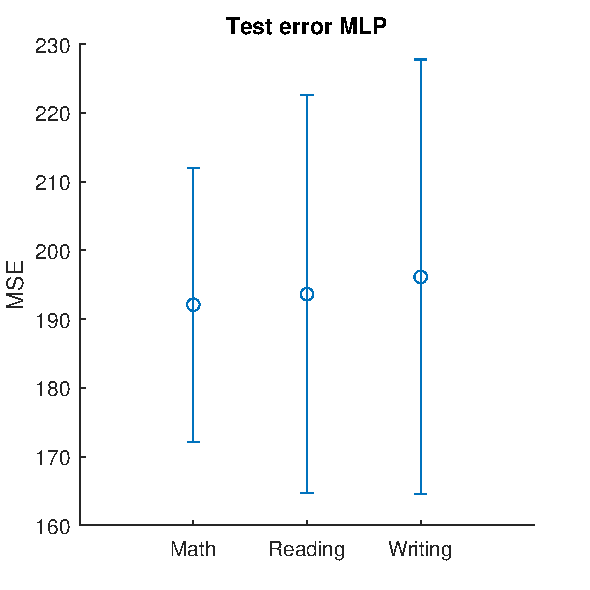
\includegraphics[height=2.2in]{purelin_purelin_50_test.png}
\caption{MSE testu dla 50 neuronów.}
\end{subfigure}
\caption{Błąd uczenia i testowania sieci dla X prób dla kolejnych egzaminów, \textbf{funkcje: purelin, purelin}.}
\end{figure}

Pierwszym omawianym zestawieniem jest prosty przykład dla kombinacji funkcji purelin oraz purelin. Otrzymane wartości błędów były jednymi z najmniejszych wśród wszystkich konfiguracji, z akceptowalnym odchyleniem. W przypadku tak prostej sieci ilość neuronów nie wpłynęła praktycznie wcale na otrzymane wyniki.

\begin{figure}[H]
\centering
\begin{subfigure}[t]{0.48\textwidth} 
\centering
\includegraphics[height=2.2in]{tansig_tansig20_learn.png}
\caption{MSE uczenia dla 20 neuronów.}
\end{subfigure}
~~
\begin{subfigure}[t]{0.48\textwidth} 
\centering
\includegraphics[height=2.2in]{tansig_tansig20_test.png}
\caption{MSE testu dla 20 neuronów.}
\end{subfigure}

\begin{subfigure}[t]{0.48\textwidth} 
\centering
\includegraphics[height=2.2in]{tansig_tansig50_learn.png}
\caption{MSE uczenia dla 50 neuronów.}
\end{subfigure}
~~
\begin{subfigure}[t]{0.48\textwidth} 
\centering
\includegraphics[height=2.2in]{tansig_tansig50_test.png}
\caption{MSE testu dla 50 neuronów.}
\end{subfigure}

\caption{Błąd uczenia i testowania sieci dla X prób dla kolejnych egzaminów, \textbf{funkcje: tansig, tansig}.}
\end{figure}
Przykładem jednej z konfiguracji, która daje mierne rezultaty jest konfiguracja z wykorzystaniem funkcji tansig oraz tansig na wyjściu. Wartości błędów były jednymi z większych, jednak istotny jest fakt, że wyniki dla trzeciego egzaminu były zbieżne, w przeciwieństwie do większości pozostałych konfiguracji. Ilość neuronów nie miała dużego wpływu na otrzymywane błędy.



\begin{figure}[H]
\centering
\begin{subfigure}[t]{0.48\textwidth} 
\centering
\includegraphics[height=2.2in]{tansig_purelin20_learn.png}
\caption{MSE uczenia dla 20 neuronów.}
\end{subfigure}
~~
\begin{subfigure}[t]{0.48\textwidth} 
\centering
\includegraphics[height=2.2in]{tansig_purelin20_test.png}
\caption{MSE testu dla 20 neuronów.}
\end{subfigure}

\begin{subfigure}[t]{0.48\textwidth} 
\centering
\includegraphics[height=2.2in]{tansig_purelin50_learn.png}
\caption{MSE uczenia dla 50 neuronów.}
\end{subfigure}
~~
\begin{subfigure}[t]{0.48\textwidth} 
\centering
\includegraphics[height=2.2in]{tansig_purelin50_test.png}
\caption{MSE testu dla 50 neuronów.}
\end{subfigure}

\caption{Błąd uczenia i testowania sieci dla X prób dla kolejnych egzaminów, \textbf{funkcje: tansig, purelin}.}
\end{figure}


Kombinacja tansig oraz purelin daje bardzo niskie wartości błędu w porównaniu z pozostałymi metodami, jednak z dość dużym rozstrzałem między otrzymywanymi wartościami. Błedy uczenia nieznacznie spadały wraz ze wzrostem ilości neuronów w warstwie, jednak tendencja dla testu była odwrotna. Najlepsze wyniki udało się uzyskać dla 20 oraz 30 neuronów.




\begin{figure}[H]
\centering
\begin{subfigure}[t]{0.48\textwidth} 
\centering
\includegraphics[height=2.2in]{radbas_tansig_purelin20_learn.png}
\caption{MSE uczenia dla  40 neuronów w pierwszej warstwie, 20 w drugiej.}
\end{subfigure}
~~
\begin{subfigure}[t]{0.48\textwidth} 
\centering
\includegraphics[height=2.2in]{radbas_tansig_purelin20_test.png}
\caption{MSE testu dla  40 neuronów w pierwszej warstwie, 20 w drugiej.}
\end{subfigure}

\begin{subfigure}[t]{0.48\textwidth} 
\centering
\includegraphics[height=2.2in]{radbas_tansig_purelin50_learn.png}
\caption{MSE uczenia dla  100 neuronów w pierwszej warstwie, 50 w drugiej.}
\end{subfigure}
~~
\begin{subfigure}[t]{0.48\textwidth} 
\centering
\includegraphics[height=2.2in]{radbas_tansig_purelin50_test.png}
\caption{MSE testu dla 100 neuronów w pierwszej warstwie, 50 w drugiej.}
\end{subfigure}

\caption{Błąd uczenia i testowania sieci dla X prób dla kolejnych egzaminów, \textbf{funkcje: radbas, tansig, purelin}.}
\end{figure}

Postanowiono również przetestować sieci o dwóch warstwach w bardziej egzotycznych konfiguracjach, dla przykładu konfiguracja radbas, tansig, purelin dała zadziwiająco niskie wartości błędów dla próby uczenia, który gwałtownie zmieniał się wraz z dokładaniem ilości neuronów. Pod względem błędu uczenia była to najlepsza konfiguracja.




\begin{figure}[H]
\centering
\begin{subfigure}[t]{0.48\textwidth} 
\centering
\includegraphics[height=2.2in]{logsig_tansig_tansig20_learn.png}
\caption{MSE uczenia dla  50 neuronów w pierwszej warstwie, 50 w drugiej.}
\end{subfigure}
~~
\begin{subfigure}[t]{0.48\textwidth} 
\centering
\includegraphics[height=2.2in]{logsig_tansig_tansig20_test.png}
\caption{MSE testu dla  50 neuronów w pierwszej warstwie, 50 w drugiej.}
\end{subfigure}

\begin{subfigure}[t]{0.48\textwidth} 
\centering
\includegraphics[height=2.2in]{logsig_tansig_tansig50_learn.png}
\caption{MSE uczenia dla  50 neuronów w pierwszej warstwie, 50 w drugiej.}
\end{subfigure}
~~
\begin{subfigure}[t]{0.48\textwidth} 
\centering
\includegraphics[height=2.2in]{logsig_tansig_tansig50_test.png}
\caption{MSE testu dla 50 neuronów w pierwszej warstwie, 50 w drugiej.}
\end{subfigure}

\caption{Błąd uczenia i testowania sieci dla X prób dla kolejnych egzaminów, \textbf{funkcje: logisg, tansig, tansig}.}
\end{figure}

Kombinacja logsig, tansig oraz tansig dała ciekawe rezultaty, wartości błędu dla wszystkich prób nie licząc trzeciego egzaminu były do siebie zbliżone. Wyniki dla trzeciego egzaminu jednak zbyt odstają od reszty, by móc brać tą konfiguracje w kolejnych badaniach.

W zestawieniu nie objęto wykresów dla pozostałych kombinacji (na przykład tansig, tansig),  gdyż niezależnie od ilości neuronów wyniki były bardzo złe.


\pagebreak
\section{Badanie wpływu ilości kolumn na wyniki sieci}
\subsection{Korelacja pomiędzy danymi}
W ramach projektu został obliczony współczynnik korelacji \textit{Pearsona} pomiędzy danymi z repozytorium. Dzięki niemu możemy sprawdzić jak bardzo zależne są od siebie dane, a dzięki temu dostosować informacje użyte do uczenia sieci.

Do obliczenia współczynnika korelacji została użyta funkcja pakietu MATLAB \verb\corr\.

\subsubsection {Korelacja pomiędzy wynikami egzaminów}
Na początku został wyznaczony współczynnik korelacji pomiędzy wynikami egzaminów. Otrzymane wyniki przedstawiono w tabeli poniżej.

\begin{table}[H]
\centering
\begin{tabular}{|c|c|c|} 
\hline
Egzamin 1 i 2 & Egzamin 1 i 3 & Egzamin 2 i 3  \\ 
\hline
0.6453 & 0.6435          &  0.8578 \\ 
\hline
\end{tabular}
\end{table}

Dla wszystkich kombinacji otrzymaliśmy wartości większe od $0.5$, możemy więc uznać, że dane są od siebie zależne. Największa korelacja występuje pomiędzy egzaminem 2 oraz 3 - współczynnik jest równy $0.86$.

Na rysunkach poniżej zależności pomiędzy zbiorami zostały przedstawione w sposób graficzny.

\begin{figure}[H]
\centering
\includegraphics[width=0.45\textwidth]{korelacja_egzamin12.png}
\includegraphics[width=0.45\textwidth]{korelacja_egzamin13.png}
\includegraphics[width=0.45\textwidth]{korelacja_egzamin23.png}
\caption{Zależności pomiędzy wynikami egzaminów przedstawione w sposób graficzny.}
\end{figure}

\subsubsection {Korelacja pomiędzy czynnikami środowiskowymi a wynikami egzaminów}
W dalszej części analizy zbioru danych została zbadana zależność pomiędzy czynnikami, będącymi wejściem sieci neuronowej, a wynikami kolejnych egzaminów. Otrzymane współczynniki korelacji przedstawiono w tabeli poniżej.

\begin{table}[H]
\centering
\begin{tabular}{|c|c|c|c|} 
\hline
 Czynnik środowiskowy & Egzamin 1 & Egzamin 2 & Egzamin 3  \\ 
\hline
Płeć & 0.1558  &  -0.1886 &  -0.2396  \\ 
\hline
Rasa &  0.1771  &  0.0770   & 0.0907 \\ 
\hline
Wykształcenie rodzica &  -0.0584  & -0.0306 &  -0.0571  \\ 
\hline
Przystąpienie do kursu & 0.3269  &  0.1906  &  0.2182  \\ 
\hline
Dieta &  -0.1564  & -0.1838   & -0.2647  \\ 
\hline
\end{tabular}
\end{table}

Otrzymane wartości są dość niskie, nie istnieje wyraźna korelacja pomiędzy którąś z tych cech, a wynikami. Najmniejszą zależność obserwujemy pomiędzy wynikami, wykształceniem rodziców - są one najbliższe zeru. Największe znaczenie ma przystąpienie do kursu przygotowawczego, w dalszej kolejności dieta oraz płeć.

% nie dałam rysunków bo by ich było za dużo, można dodać potem jak uważasz że jakiś
% no np dla tych największych korelacji/najmniejszych

\subsection{Testowanie sieci neuronowej z pomniejszonym zbiorem uczącym}
Dla wybranych najlepszych parametrów sieci zostało przeprowadzone uczenie ze zmniejszoną ilością kolumn. Celem tego zabiegu było zbadanie, jaki wpływ mają te czynniki na poprawność działania sieci. %to jest nie po polsku xd

\pagebreak
\section{Przewidywanie wyniku bazując wynikach pozostałych egzaminów} %to też źle brzmi
Jak zostało zauważone podczas badania korelacji, wyniki egzaminów są od siebie zależne (wysoki współczynnik korelacji). Korzystając z wyników z dwóch egzaminów podjęto próbę stworzenia sieci obliczającą wynik z trzeciego egzaminu.

Otrzymane błędy testowania zostały przedstawione poniżej.

% rysunki z MSE oraz obok taki rysunek że jakie powinny być i jakie były przewidziane
\begin{figure}[H]
\centering
\includegraphics[width=0.45\textwidth]{cz3_egz_ucz.png}
\includegraphics[width=0.45\textwidth]{cz3_egz_test.png}
\caption{Błąd uczenia i testowania sieci dla X prób dla kolejnych egzaminów}
\end{figure}

Na podstawie obserwacji wielkości błędów, można zauważyć, że dla egzaminów 2 oraz 3 sieć osiąga dobre wyniki - na poziomie wartości $50$.  Przeprowadzono badanie błędu średniokwadratowego dla uczenia oraz testu różnych konfiguracji funkcji aktywacji, ilości warstw oraz ilości neuronów w poszczególnych warstwach.


Otrzymane wyniki można powiązać z analizowaną wcześniej korelacją danych - wyniki egzaminów 2 i 3 są ze sobą w większym stopniu powiązane, niż egzamin 1 z egzaminem 2 lub 3.

% to że błędy są mniejsze niż na podstawie czynników środowiskowcyh

%  w sumie można ejszcze zrobić (jak zostanie czas) uczenie czynnikami + wynik pozostałych egzaminów, powinno być najlepiej

\pagebreak
\section{Podsumowanie}
% wnioski

\pagebreak

\begin{thebibliography}{9}


\end{thebibliography}

\end{document}